\documentclass[conference]{IEEEtran}
\usepackage{cite}
\usepackage{amsmath}
\ifCLASSINFOpdf
  \usepackage[pdftex]{graphicx}
   \DeclareGraphicsExtensions{.pdf,.jpeg,.png}
\else
 \fi
 
% correct bad hyphenation here
\hyphenation{op-tical net-works semi-conduc-tor}


\begin{document}
%
% paper title
% can use linebreaks \\ within to get better formatting as desired
% Do not put math or special symbols in the title.
\title{Dynamic Rendezvous based Routing Algorithm on Sparse Opportunistic Network Environment}


% author names and affiliations
% use a multiple column layout for up to three different
% affiliations
\author{\IEEEauthorblockN{Jiradett Kerdsri}
\IEEEauthorblockA{School of Information, Computer, \\and Communication Technology (ICT), \\Sirindhorn International Institute of Technology, Thailand
%\IEEEauthorblockA{ Defense Technology Institute \\(Public Organisation) Ministry of Defense, \\Nontburi, Thailand
\\Email: jiradett.k@dti.or.th}
\and
\IEEEauthorblockN{Komwut Wipusitwarakun}
\IEEEauthorblockA{School of Information, Computer, \\and Communication Technology (ICT), \\Sirindhorn International Institute of Technology, Thailand
\\Email: komwut@siit.tu.ac.th}
}

% make the title area
\maketitle

% As a general rule, do not put math, special symbols or citations
% in the abstract
\begin{abstract}
Opportunistic network is a challenge network where the nodes need to communicate with each other even either direct or indirect routes between them may not permanently exist due to the nodes' random movement.
Most routing algorithms in this dynamic network environment employ \textit{store-carry-forward} paradigm by which a node can keep the receiving messages, carrying the messages with them when moving and then forwarding the messages (or the copies) to the opportunistic meeting nodes when possible.
This routing model works well in the networks with high-to-moderate node density in which the opportunity that the moving nodes can meet with each other is rather high.
On the other hand, it has been reported that the delivery ratio becomes remarkably low in the sparse network environment especially when there is strict constraint on message delivery deadline.
In this paper, we introduce the novel concept of rendezvous place where the passing nodes can announce, deposit or pickup their own messages without having to meet the other nodes carrying the desired message. 
In the proposed scheme, the rendezvous place can be detected automatically and its area's size and shape are dynamically changed according to the interaction among nodes passing around the area.
The results from intensive simulations show that our proposed routing algorithm can achieve higher delivery ratio and utilize lower energy consumption than traditional opportunistic routing algorithms especially in sparse network environment.

\end{abstract}
\IEEEpeerreviewmaketitle



\section{Introduction}
%What is OppNet?
Opportunistic Network (OppNet) is an extreme type of Delay Tolerant Networks (DTNs) where the source and destination nodes might never be fully connected at the same time, thus there is no guarantee on the existence of a complete path between two nodes wishing to communicate \cite{MWNsBook2011}.
This intermittent connections may result from several factors such as high node mobility, low node density, environmental interference and obstruction, short radio range and malicious attacks \cite{prodhan2011} etc.
The node movement in OppNet is extremely random in some networking environment, thus the probability of message delivery from source to destination is difficult to assure.
Example of such networks are sparse mobile ad hoc network \cite{Alekeish2012}, military tactical networks \cite{Scott2005,Kerdsri2013}  or sensor networks, such as ZebraNet \cite{zebranet2004}, SWIM \cite{Small2003}  which are wireless sensor networks in which nodes move throughout an environment working to gather and process information about their surroundings.
Commonly, the key differentiating factors among those scenarios are the amount of predictability and control over the contacts between the message carriers\cite{Karkkainen2013}.
%Algorithms --> Store Carry Forward
A key concept behind Opportunistic Routing (OR) is overhearing and cooperation among relaying nodes to overcome the drawback of unreliable wireless transmission \cite{Liu2009}.
Since the mobile nodes are not always connected to each other, the forwarding algorithms in such network commonly follow a store-carry-forward (SCF) paradigm.
This SCF employs storage space and node mobility to overcome the intermittent connectivity \cite{Ma2011}.
The messages sent from the source node are carried by intermediate nodes to other geographical area and transfered to adjacent nodes until the destination node receives this message.
%From part A
Since this fundamental SCF routing model realistically requires a certain sufficient occasion of \emph{direct} encounter among moving nodes to exchange messages, its routing performance will highly degrade in the low-node-density sparse network \cite{Spyropoulos2010}.
%From part A2
Although there are several existing OppNet routing solutions \cite{ Zhang2013, Chung-Ming2008, Spyropoulos2004, Grossglauser2002, Vahdat2000,Kerdsri2013} proposed in the literature, very few proposals address the problem in this sparse network environment especially when the OppNet nodes are energy-constrained \cite{Liguang2013,Eu2010} and the direction of their movement cannot be controlled.
One interesting application of such OppNet environment is the sensor OppNet for wildlife monitoring and tracking \cite{zebranet2004, Small2003}.

%From part B
In this paper, we proposed a novel Dynamic Rendezvous based Routing Algorithms (DRRA) to increase message exchanging opportunity even in the sparse network environment.
We utilize the fact that there should be some node-gathering (Rendezvous) places forming somewhere at some specific time in the real network.
These Rendezvous places may be either predictable such as along the river in the wildlife monitoring application, or non-predictable such as disaster and emergency networks.
An energy constrained node should maximize its resource usage to communicate with the others only when entering into the rendezvous area.
In the proposed scheme, the rendezvous place is dynamically marked by the help of a special controllable Rendezvous node and the proposed rumor protocol to let nodes in the rendezvous area exchange messages more efficiently without having to directly meet with the other nodes.

The rest of the paper is organized as follows. 
In section II, we discuss the  overview of SFC routing models and existing works. 
The detail of rendezvous based routing model is elaborated in section III.
In section IV, we present the result of our simulation and show the performance of our scheme under different conditions.
We conclude the paper and point out some future research directions in section V.   


\section{The SCF routing models and existing works}
\begin{figure}[!t]
	\centering
	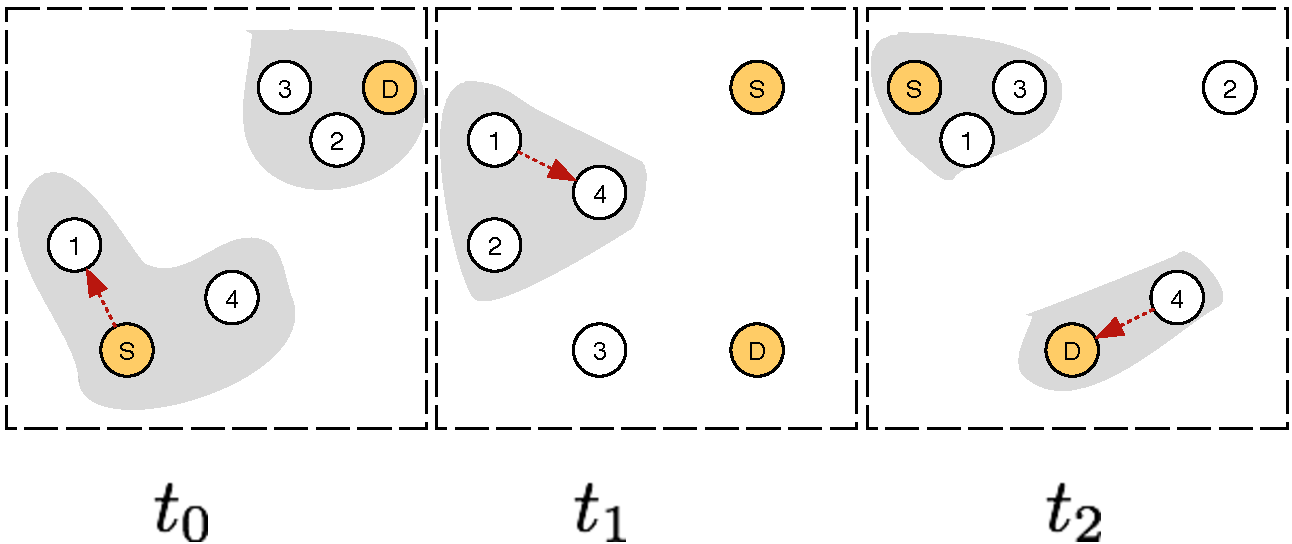
\includegraphics[width=3in]{Figures/SFC.pdf}
	\caption{Store Carry and Forward routing model}
	\label{SFC}
\end{figure}

In OppNet, the messages are delivered using Store-Carry-Forward routing by which  the nodes can exchange data whenever they come in close.
If there is no direct connection from source to destination, data holding nodes will discover their nearest neighbor nodes to forward messages toward the destination node as shown in Fig. \ref{SFC}.
There are several existing works in the literature \cite{Vahdat2000, Harras2005, Neena2013, Lindgren2003,Brendan2005,Boldrini2007,Kerdsri2013} with the aim for 100\% delivery ratio which is quite difficult to achieve especially in sparse network with constraints in energy consumption and message delivery deadline.

Vahdat et al \cite{Vahdat2000} proposed the epidemic routing using  uncontrolled flooding algorithm in which the replication of source data is not restricted with any limits in order to route the message from source to destination in the intermittently connected network.
However, this type of routing incurs significant demand on both bandwidth and buffer.
To address the excess traffic overhead, Khaled et al \cite{Harras2005} proposed a Controlled Flooding  scheme which can limit the flooding by three parameters: Willingness probability, Time-to-Live, and Kill Time.
Nevertheless, flooding based routing performance degrading has been reported in a very sparse network \cite{Neena2013}.

Lindgren et al \cite{Lindgren2003} proposed a prediction based routing called PROPHET (Probabilistic Routing Protocol using History of Encounters and Transitivity) by estimating the delivery predictability to indicate the probability of success in delivering a message to the destination from the local node.
In this prediction based routing category, Brun et al \cite{Brendan2005}  also proposed a protocol utilizing the motion vector of mobile nodes to predict the future location of mobile nodes by using the knowledge of relative velocities of a node and its neighbor nodes to predict the closest distance between two nodes.
Although the prediction based approach can reduce traffic overhead in the network, but it lacks of the aim to improve the performance in extremely low node density and failed in some certain cases which leads to the delivery ratio reduction.

To refine the prediction based routing,  Boldrini et al \cite{Boldrini2007}  proposed the History based routing (HiBOp) which exploits current context information for data forwarding decisions.
Even though, this context based routing approach can reduce the resource consumption in terms of network traffic and storage but it increases the delay which results in significantly less efficient than Epidemic algorithm.
%In our work of content based routing, DORSI protocol \cite{Kerdsri2013} aims to differentiate the messages by their significant in order to improve the delivery ration of important data.
Kerdsri et al \cite{Kerdsri2013} proposed DORSI protocol with the concept of content based routing which aims to classify the data in the network by messages' significance level in order to guarantee the delivery of more important data. 
However, the decreasing in network performance under sparse environment is not mentioned in this proposed protocol.
Overall, the performance of most existing algorithms are degrading in very sparse node density and the energy consumption does not take in to the consideration which is a crucial factor in such mobile sensor devices such as in wildlife monitoring.


\section{The proposed Rendezvous based OppNet system}

\subsection{System model}
\begin{figure*}[!t]
	\centering
	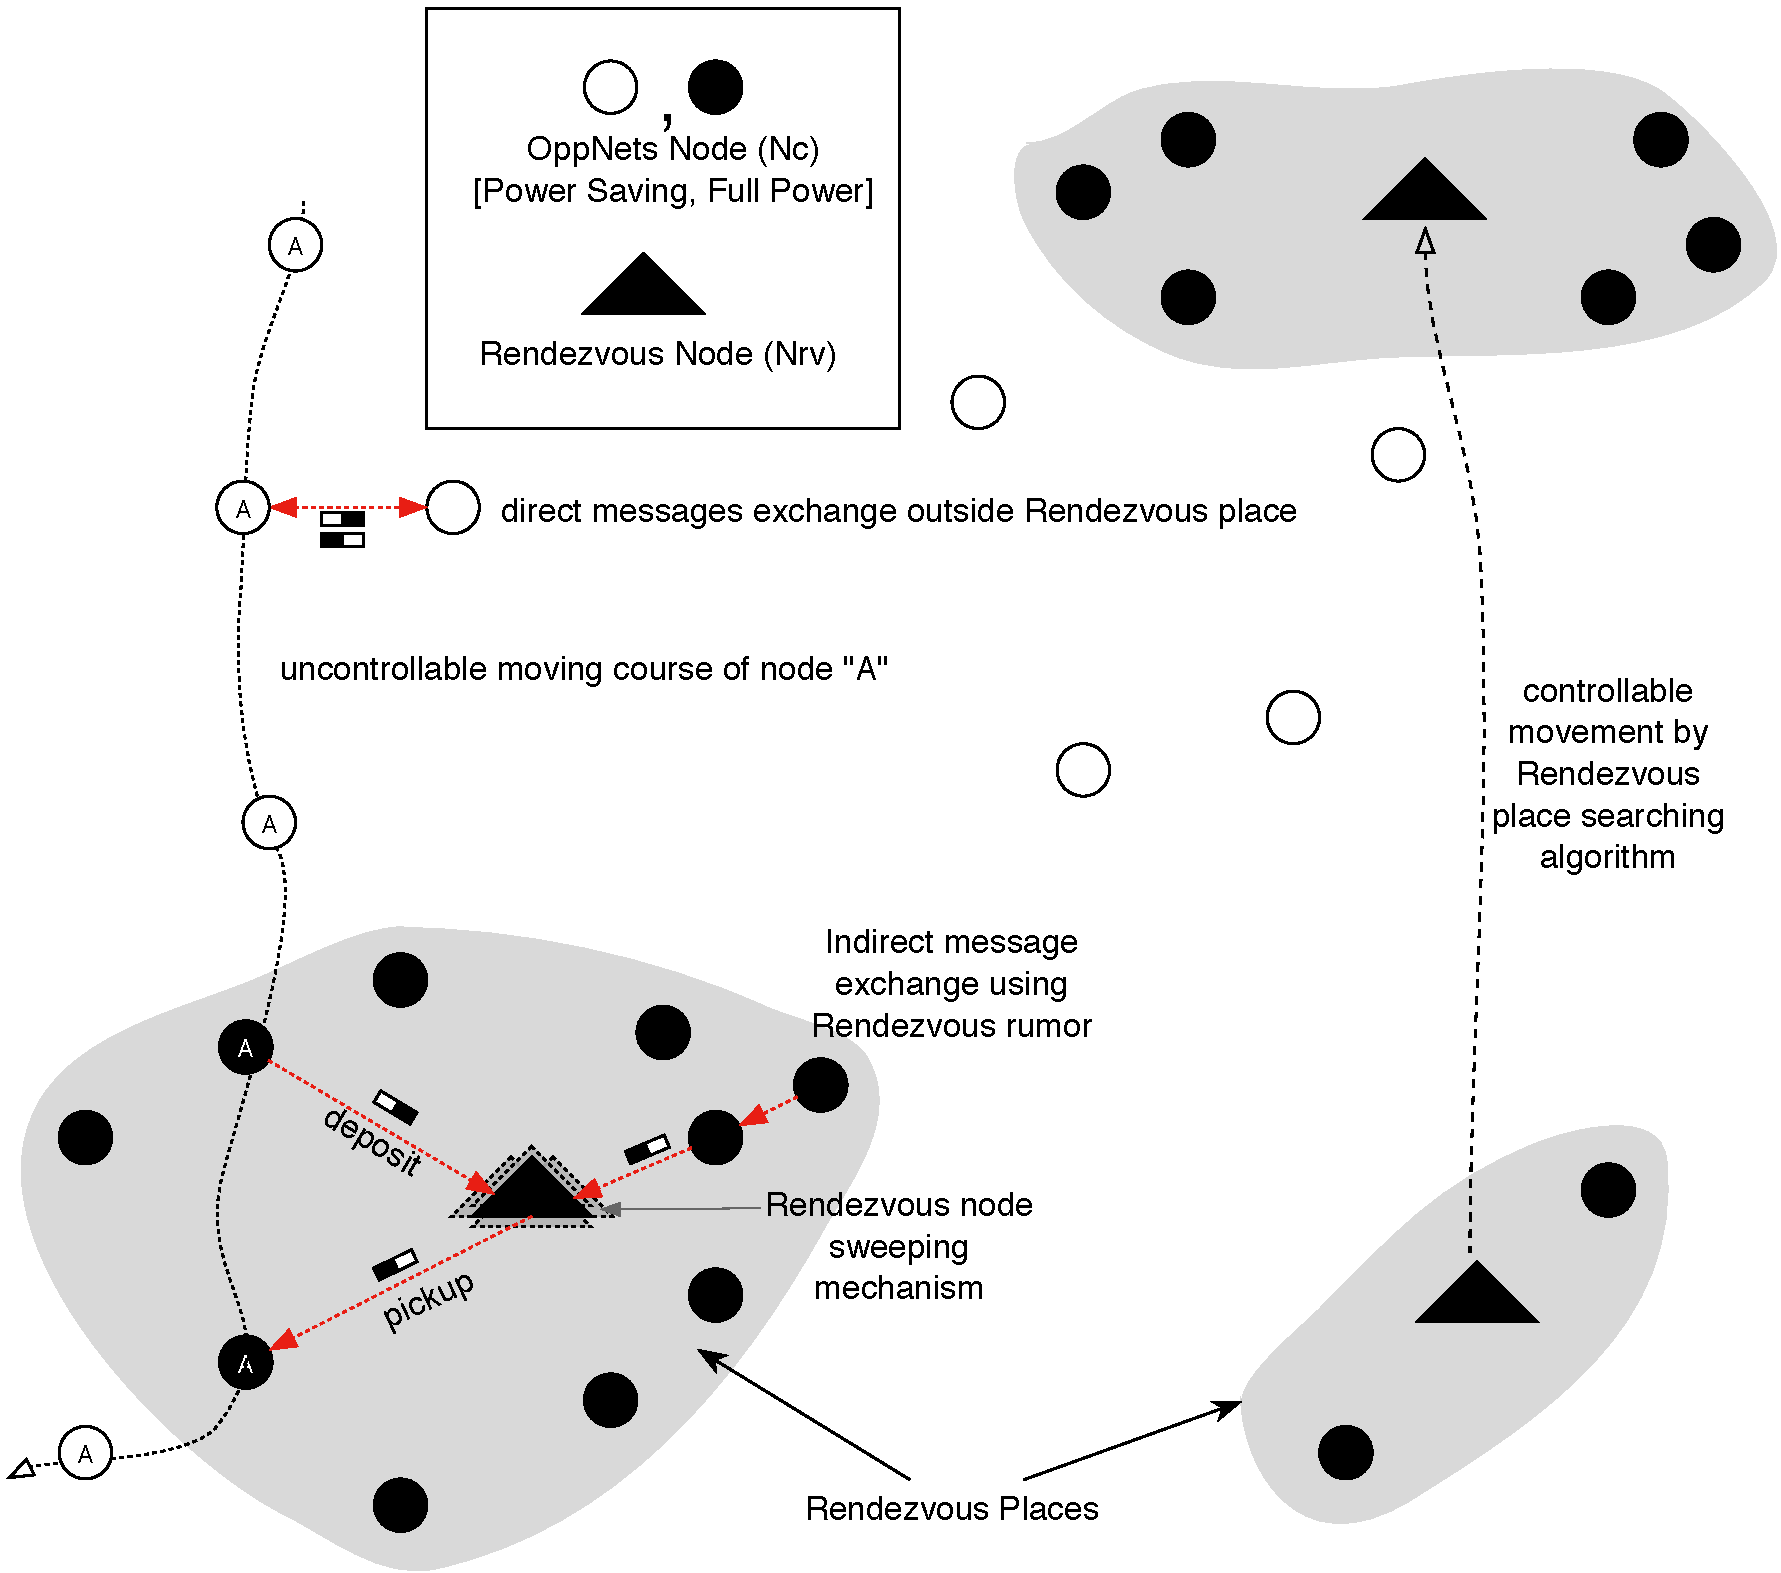
\includegraphics[width=5.5in]{Figures/NewSystemModel.pdf}
	\caption{System model}
	\label{System model}
\end{figure*}

The proposed system is designed to efficiently use the node-gathering area, i.e. Rendezvous place, for depositing the delivered messages as much as possible so that the messages can be picked up by the destination node without requiring the exact timing of direct contact between the node carrying a message and the desired destination node.
In addition, all nodes should reserve its energy as much as possible when they are out of the Rendezvous area.

As shown in Fig. \ref{System model}, the OppNet node, $N_{c}$, whose movement direction is uncontrollable, moves in the system using \textit{Power Saving Mode}  until it reaches the Rendezvous place where it will turn itself to \emph{Full Power Mode} in order to announce its arrival, deposit its carried messages and pick up the messages destined to itself, to/from the Rendezvous place.
The Rendezvous Rumor protocol and Rendezvous Node Sweeping mechanism are used inside the Rendezvous area to let messages being exchanged more effectively without the need of direct contact between the OppNet node and the high-resource direction-controllable Rendezvous node, $N_{rv}$, which is act as the center of the Rendezvous place.
The Rendezvous nodes will move around the OppNet network to create suitable Rendezvous places according to the proposed \emph{Rendezvous Place Searching algorithm}.

\subsection{OppNet node's operational modes: "Full Power" and "Power Saving"}
The OppNet node ($N_{c}$) is a mobile node equipped with the radio interface whose transmission rage is adjustable in range of $[{ r }_{ c }^{ min },{ r }_{ c }^{ max }]$.
The node will operate in either \emph{Full Power mode} or \emph{Power Saving mode} according to its location.
\subsubsection{Full power mode}
In this mode, the node will use its full transmission power, ${ r }_{ c }^{ max }$, to search for nearby nodes and exchange messages.
It will switch to this mode only when getting into the Rendezvous area.

\subsubsection{Power saving mode}
The node, by default, operates in this mode if it is outside the Rendezvous place.
In this mode, it will alternately change its transmission range between ${ r }_{ c }^{ min }$ and ${ r }_{ c }^{ max }$ in the process of searching for nearby nodes.
However, if it receives the searching signal from the other node, it will switch to its full ${ r }_{ c }^{ max }$ immediately in order to increase opportunity to exchange messages with the encountered node as much as possible.
Then, it will switch back to minimum ${ r }_{ c }^{ min }$ when departing from the communicating node.
Besides the ${ r }_{ c }^{ min }$ and ${ r }_{ c }^{ max }$ values, the ratio of the time interval being in it full ${ r }_{ c }^{ max }$ over the whole time period is a configurable parameter,$\tau_{s}$ , as shown in Fig. \ref{Operational modes}.

\begin{figure}[!t]
	\centering
	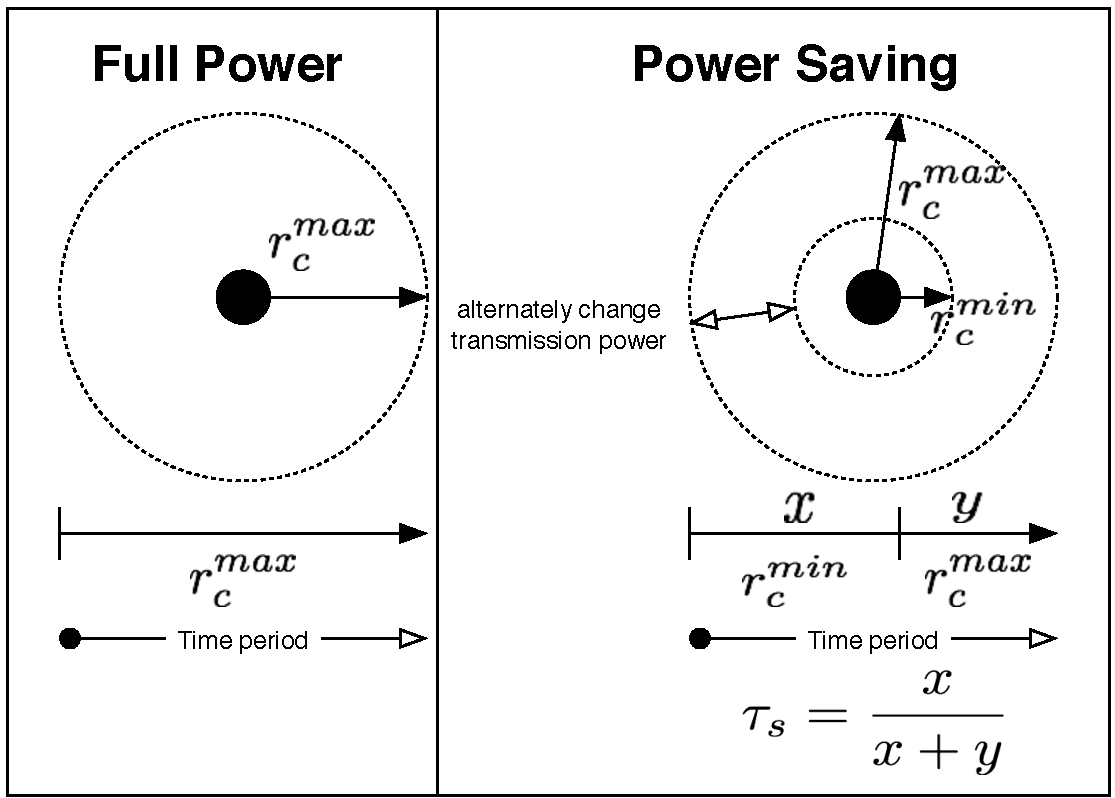
\includegraphics[width=3in]{Figures/OperationalMode.pdf}
	\caption{Operational modes}
	\label{Operational modes}
\end{figure}



\subsection{Rendezvous place and its Rumor protocol}

The Rendezvous place is a dynamic area centered by a special controllable Rendezvous node, $N_{rv}$.
This $N_{rv}$ node is full of resources such as large message storage and high radio power with maximum transmission range $R_{rv}$.
The Rendezvous place is controlled by the Rendezvous node using Rendezvous rumor protocol.

The area in Rendezvous place is not fixed as the maximum radio range, $R_{rv}$,  of the Rendezvous node, instead it is virtually determined by the covering radio range of the most outer OppNet nodes which can relay the data messages from the Rendezvous node, as shown in Fig. \ref{System model}

When an OppNet node detects the \emph{Rendezvous Area rumor message} $(RA)$ broadcasted from the Rendezvous node, it learns that it enters to the Rendezvous area.
Then, it will switch its operational mode to \emph{Full Power mode} and try to rebroadcast such \emph{Rendezvous Area }rumor message so that the other reachable nearby nodes can learn about Rendezvous place and can adaptively expand the area on-demand.
Additionally, the OppNet node in the Rendezvous area will periodically announce its arrival and upload its carried data messages to the Rendezvous node via the \emph{Keep-Alive} rumor message $(KA)$ and the \emph{Deposit} rumor message $(DP)$ respectively.
Note that all types of rumor messages will be automatically repeated with \emph{duplication filtering} function throughout the area by other OppNet nodes.

Once the rendezvous node receives the \emph{Keep-alive} rumor message which contains the sending node ID, it will gather all data messages destined to the node ID from its message storage, encapsulate those found messages into the created \emph{Pick-up} rumor message and then broadcast the \emph{Pick-up} message $(PU)$ throughout the Rendezvous area.
On the other hand, the Rendezvous node will keep all of data messages contained in the received \emph{Deposit} rumor messages in its storage for later sending out to the area when the target node appears later as seen in Fig. \ref{Rendezvous Place}. 

In addition to the Rendezvous rumor protocol, the Rendezvous node implements the rumor message sweeping algorithm in order to increase the chance to collect as many rumor messages as possible.
Instead of always being stationary at the center location of the Rendezvous place, the rendezvous node will periodically move to its four directions (North, East, West, South) by the distance of its radio transmission range as shown in Fig. \ref{Sweep mechanism}.
This design lets the OppNet nodes on the edge of Rendezvous node's radio range, whose radio signal may not reach to the Rendezvous node due to the difference in their radio transmission range, can speak back to the Rendezvous node.

\begin{figure}[!t]
	\centering
	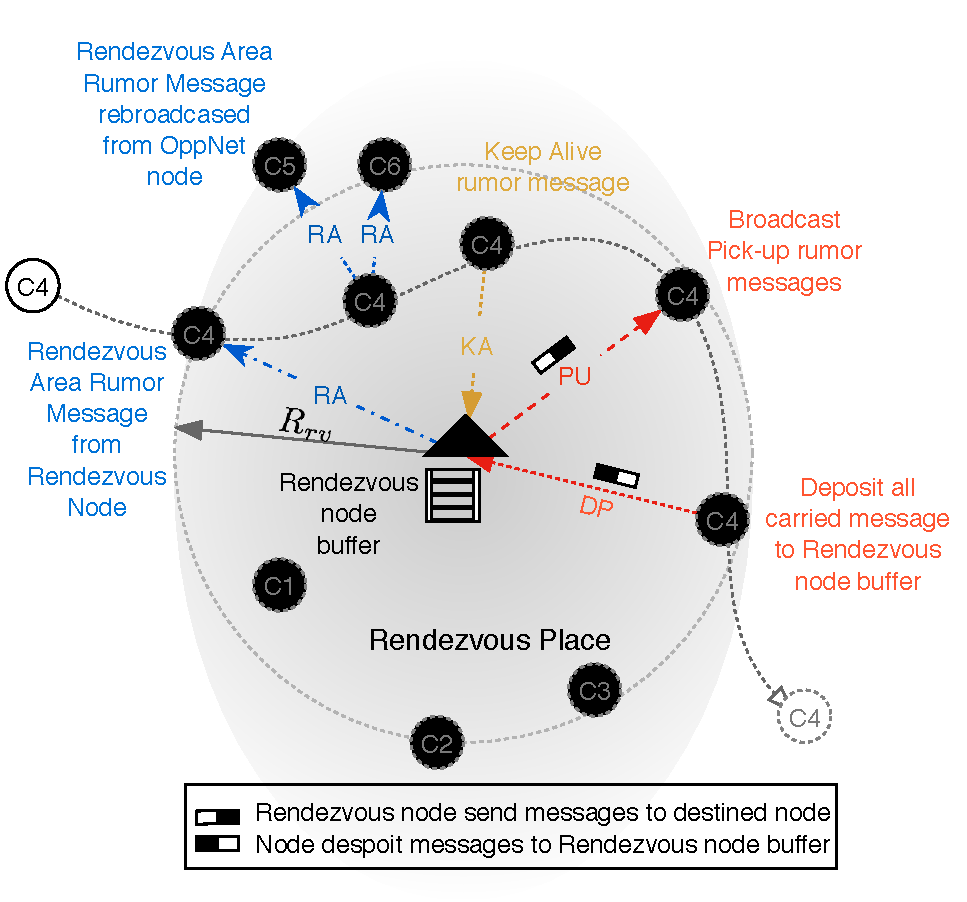
\includegraphics[width=3.5in]{Figures/NewRendezvousPlace.pdf}
	\caption{Rendezvous Place}
	\label{Rendezvous Place}
\end{figure}


\begin{figure}[!t]
\centering
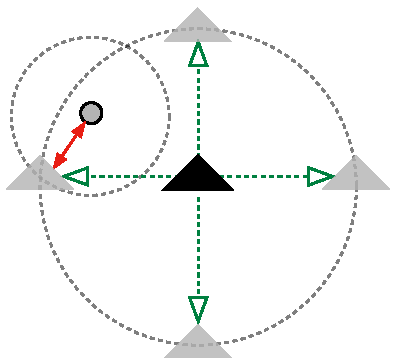
\includegraphics[width=1.5in]{Figures/Sweep.pdf}
\caption{Sweep mechanism}
\label{Sweep mechanism}
\end{figure}

\subsection{Rendezvous place searching algorithm}
In the proposed system, the Rendezvous node should move to find the node-gathering area corresponding with the real behavior of OppNet node.
\begin{figure}[!t]
	\centering
	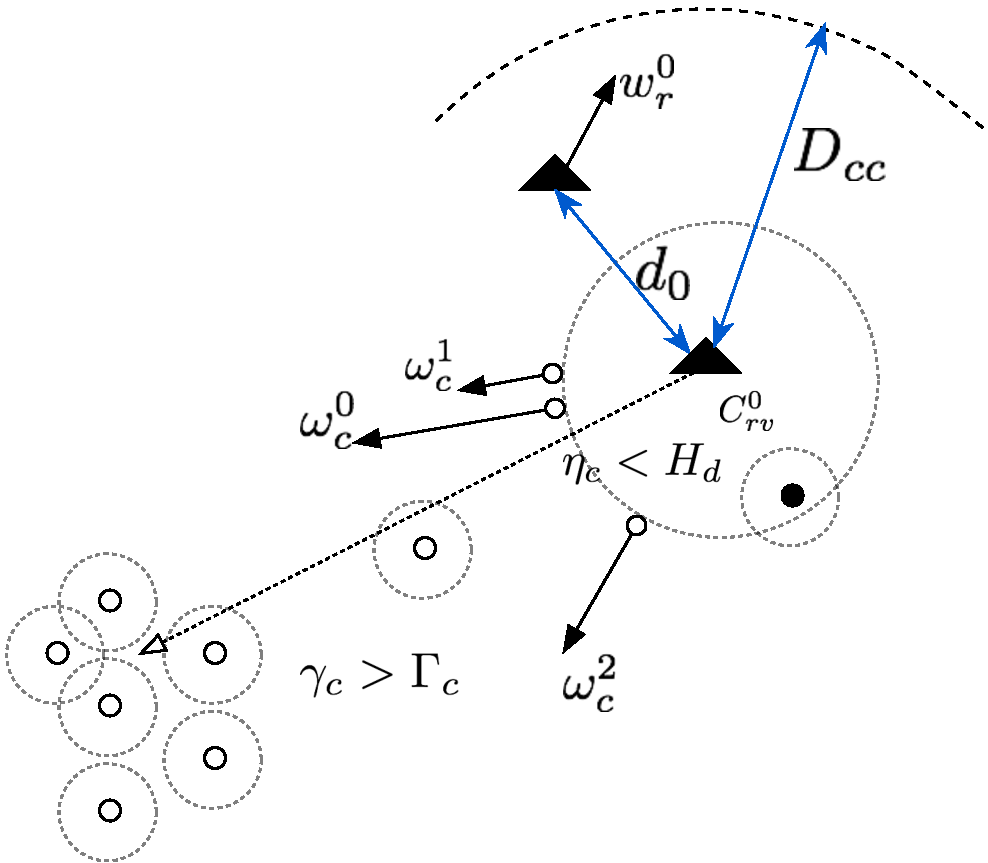
\includegraphics[width=2.5in]{Figures/Dynamic.pdf}
	\caption{Rendezvous place searching}
	\label{Rendezvous node movements}
\end{figure}
\subsubsection{Predictable behavior OppNet nodes}
In some applications, the movement of OppNet node is somehow predictable.
Take a wildlife monitoring as an example, most animals are usually cyclically gathering in the high supplies area such as along side of the main river of some specific place at some specific time \cite{Yu2007}.
In these applications, the Rendezvous nodes can be programmed to be located at those areas at the proper time in order to maximize the effectiveness of the proposed system.

\subsubsection{Non-Predictable behavior OppNet nodes}
Without any priori knowledge about OppNet node, the proposed \emph{dynamic Rendezvous Place Searching Algorithm} can be used to guide the Rendezvous nodes to the node-gathering area.
The Rendezvous node will decide to move to the new node gathering location if the number of OppNet node in the current Rendezvous place ($\eta_{c}$) falls below the predefined departure node threshold, $H_{d}$.
The movement direction, $\vec{\Delta}$, will be determined periodically based on the collected statistical data from both previously contacting OppNet nodes and other neighboring Rendezvous nodes as in Eq.\ref{DirectionParameter}.
In the equation, $\vec{w_c}$ is the departure directional unit vector of the contacted OppNet nodes, $\vec{w_r}$ is the directional unit vector of the other Rendezvous nodes and the $\varphi$ is a configurable weighting factor between group of OppNet nodes and group of other Rendezvous nodes in the area.

\begin{eqnarray}
\label{DirectionParameter}
\vec{\Delta} =\sum _{ i=1 }^{ C }{ \vec { { \omega }_{ c }^{ i } }  } + \varphi \sum _{ j=1 }^{ R }{ \delta\left( d_{j} \right)
	\vec { {w }_{ rv }^{ j } }  }
\end{eqnarray}

While the $\delta\left( d_{j} \right)$ is the on-off function to include only the other Rendezvous nodes whose distance $d_j$ is the range of cut-off distance perimeter, $D_{cc}$, and the  $C$ and $R$ are the number of contacted OppNet nodes and the number of other Rendezvous nodes respectively.

\[\delta \left( { d }_{ j } \right) =\begin{cases} 1\quad ;\quad { d }_{ j }\quad \le { \quad D }_{ cc } \\ 0\quad ;\quad { d }_{ j }\quad >{ \quad D }_{ cc } \end{cases}  \] 

The Rendezvous node will decide to stop at the expected node-gathering area when the number of OppNet nodes in the current Rendezvous place ($\gamma_{c}$) become greater than the predefined Rendezvous place node threshold, $\Gamma_{c}$ as shown in Fig. \ref{Rendezvous node movements}.  

%%%%%%%%%%%%%%%%%%%%%%%%%%%%%%%%%%%%%%%%%%%%%%%%%%%%%%%%%%%%%%%%%%%%%%%
\section{Evaluation}
%%%%%%%%%%%%%%%%%%%%%%%%%%%%%%%%%%%%%%%%%%%%%%%%%%%%%%%%%%%%%%%%%%%%%%%
The objective of the evaluations is to analyze the performance of our proposed protocol on the sparse network environment comparing with traditional OppNet protocols.
We compare both predictable and non-predictable behavior OppNet nodes with the commonly well-known Epidemic protocol\cite{Vahdat2000} under different node density environments.

%%%%%%%%%%%%%%%%%%%%%%%%%%%%%%%%%%%%%%%%%%%%%%%%%%%%%%%%%%%%%%%%%%%%%%%
\subsection{Simulation setup}
We setup a simulation environment using ONE (Opportunistic Network Environment) \cite{Keranen2009b}, which is a powerful tool designed for running opportunistic network simulation with various routing protocols and different movement models.
%%
All the results are obtained by averaging over a few hundreds independent simulation runs with different seeds.
%%
For the OppNet simulation model, the main parameter that largely effected the evaluation performance is the movement model.
%%
In our evaluation, we deploy Group movement model instead of the most commonly used, Random Way Point (RWP) model \cite{Batabyal2012}, to correctly capture the the actual behavior of node movements.
%%
In fact, several multi-hop wireless network scenarios are most realistically represented using Group movement model \cite{Blakely2004} which represents the random motion of a group of mobile nodes as well as the random motion of each individual mobile node within the group.
%%
This is the vital case for modeling the routing simulation in OppNet since the movements in several cases are in swarm behavior, in which nodes are aggregating together and moving in some directions, such as the movement of animals or military tactical operations.
%%
The other parameters that mainly effect the evaluation performance are the area of operation, the wireless range of the nodes, node velocity and spatial location of the nodes \cite{Batabyal2012}. 
%%
In our simulation, we fix the number of nodes while increasing and decreasing the area of operation which results in wide range of node density parameter for evaluation.
%%
Node density ($\lambda$) is defined as the number of nodes per unit area. 
If $N$ nodes are distributed in a square grid of size $M \times M \quad{ m }^{ 2 }$ then the $\lambda$ is given by $\lambda =\frac { N }{ { M }^{ 2 } } $ . 
%%
The wireless range of our OppNet node can be adjusted depending on the environment while the node velocity is equal to the normal human walking speed.
%%
The common parameters are summarized in Table \ref{table_parameters}.

%%%%%%%%%%%%%%%%%%%%%%%%%%%%%%%%%%%%%%%%%%%%%%%%%%%%%%%%%%%%%%%%%%%%%%%
\subsection{Metric}
\begin{table}[!t]
	\renewcommand{\arraystretch}{1.3}
	\caption{simulation variables}
	\label{table_parameters}
	\centering
	\begin{tabular}{|c|c|c|}
		\hline
		Parameters         &  $N_{c}$ & $N_{rv}$ \\ \hline
	%	Simulation Time     & \multicolumn{2}{|c|}{10800 Seconds }  \\ \hline
		Message Size       &  \multicolumn{2}{|c|}{500 KB - 1 MB}        \\ \hline
		% Node Buffer         & \multicolumn{2}{|c|}{500 MB}&  10 GB      \\ \hline
		Maximum Radio Range & 30 Meters  & 100 Meters \\ \hline
		Transmission Speed &  \multicolumn{2}{|c|}{ 54 Mbps   }        \\ \hline
		Router             & \multicolumn{2}{|c|}{ DRRA | Epidemic   } \\ \hline
		Moving Speed       &   \multicolumn{2}{|c|}{0.5 - 1.5 m/s }        \\ \hline
		Movement Model     &   \multicolumn{2}{|c|}{Group Movement Model  }      \\ \hline
	\end{tabular}
\end{table}

Opportunistic routing protocols are commonly evaluated by delivery ratio, median latency and network overhead.
%%
In this paper, we focus on delivery ratio and network overhead in term of energy consumed to deliver a message within a specific message deadline.
%%
We assume that all messages delivered within the deadline has no difference in protocol performance.

% Opportunistic routing protocols are commonly evaluated by delivery ratio, median latency and network overhead.
% However, we required specific composite metrics in order to clearly observe the performance of our proposed protocol.
% In our evaluation we consider the following metrics:

\paragraph{Delivery ratio ($D_{r}$)} is defined as the ratio of the total number of messages successfully delivered within the deadline ($ { M }_{ delivered }$) to the total number of messages created from the source nodes that need to be delivered ($ { M }_{ created }$) as shown in Eq. \ref{delivery_ratio}.

	\begin{equation}
	\label{delivery_ratio}
	D_{r} =\frac { { M }_{ delivered } }{ { M }_{ created } } 
	\end{equation}

\paragraph{Energy consumption ($E_{c}$)} is defined as the amount of energy consumption required by all related OppNet nodes to deliver one $M_{created}$ message.
%all $M_{created}$ messages.
%%
% We simplify the energy consumption model by only considering for the communication energy consumption of the wireless interface to transmit all necessary protocol packets, $M_{packet}$.
We simplify the energy consumption model by only considering for the communication energy consumption of the wireless interface to transmit a message by determining the number of all necessary protocol packets, $M_{packet}$ per number of $M_{created}$ messages.
%%
To transmit an $L$ bit-length packet using radio interface with transmission length, $d$, the consumed energy, ${ E }_{ T }$, can be determined by Eq.\ref{eq:enegy} \cite{Yang2010, Wang2006}, where $\alpha$ is the power loss component with $\alpha \in \left[ 2,4 \right]$ and $\epsilon { f }_{ s }\left[ J/(bit/{ m }^{ \alpha  }) \right]$ is the amount of energy consumed by an amplifier to transmit one bit data at an acceptable quality level.

\begin{IEEEeqnarray}{rCl}
	\label{eq:enegy}
	{ E }_{ T }\quad =\quad L\cdot  { \epsilon  }_{ fs } \cdot  { d }^{ \alpha  }
\end{IEEEeqnarray} 

As a result, the energy consumption ($E_c$) can be derived as Eq. \ref{eq:enegy_consumed} 

\begin{IEEEeqnarray}{rCl}
	\label{eq:enegy_consumed}
	{ E }_{ c }\quad =\quad \frac{M_{packet}}{M_{created}} \cdot L_p \cdot  { \epsilon  }_{ fs } \cdot  { r }^{ 2 }
\end{IEEEeqnarray} 

Note that $L_p$ is the size of protocol packet, $r$ is the radio transmission range of the protocol packet and $\alpha$ is equal to two in our simulations.
%%
\paragraph{Protocol performance ($P_{\Psi}$)} is a composite metric to capture the gain in both delivery capability and energy saving capability of a specific protocol, compared with the baseline protocol, Epidemic.
%%
The $P_{\Psi}$ can be calculated from Eq. \ref{eq:protocol_performance}.

\begin{eqnarray}
\label{eq:protocol_performance}
{ P }_{ \Psi }= {{ D }_{ r }^{ P,B }} \cdot \frac { 1 }{ { E }_{c}^{ P,B } } 
= \frac {{ D }_{ r }^{ P }}{{ D }_{ r }^{ B } } \cdot \frac{{ E }_{c}^{ B }}{{ E }_{c}^{ P }}
\end{eqnarray}



% \paragraph{Protocol performance ($P_{p}$)} is a composite metrics defined as a delivery ratio per energy consumption unit in order to clearly analyze our protocol performance.
% Basically, the relation between energy consumption and radio range can be determined by Eq.\ref{eq:enegy} \cite{Yang2010, Wang2006}.

% \begin{IEEEeqnarray}{rCl}
% 	\label{eq:enegy}
% 	{ E }_{ T }\quad =\quad M_{packet}\cdot L\cdot  { \epsilon  }_{ fs } \cdot  { r }^{ \alpha  }
% \end{IEEEeqnarray} 

% ${ E }_{ T }$ is the amounts of transmission energy consumed at a node for transmitting an L-length message, 

% where $\alpha$ is the power loss component with $\alpha \in \left[ 2,4 \right]$ and $\epsilon { f }_{ s }\left[ J/(bit/{ m }^{ \alpha  }) \right]$ is the amount of energy consumed by an amplifier to transmit one bit data at an acceptable quality level.


% In this protocol, we approximately determine the relationship between unit of consumed energy and radio radius of node in the term of exponential equation.
% We assume the simplicity of energy model by only accounting for the communication energy consumption of a wireless interface and do not consider other resources such as computation, location services or mobility.
% In fact, the messages generated from protocol are accounted for the protocol performance.
% As a result, the energy consumption can be simply derived as Eq. \ref{eq:new_energy}.

% \begin{eqnarray}
% 	\label{eq:new_energy}
% 	{ E }_{ P }\quad \propto { \quad M }_{P }\cdot{ r }_{ P }^{ 2 }
% \end{eqnarray}

% Therefore, the protocol performance can be calculated from  Eq. \ref{eq:protocol_performance}.

% \begin{eqnarray}
% \label{eq:protocol_performance}
% { P }_{ P }=\frac { { D }_{ r }^{ P,B } }{ { E }_{ P,B } } =\frac { { D }_{ r }^{ P }/{ D }_{ r }^{ B } }{ \left( \frac { { M }_{ P }{ \cdot r }_{ P }^{ 2 } }{ { M }_{ B }\cdot { r }_{ B }^{ 2 } }  \right)  } 
% \end{eqnarray}

In this Equation, $P$ is the target protocol while $B$ is the baseline protocol (Epidemic protocol, for example) to be used as comparative energy reference.
% $M$ is the message number transmitted by OppNet nodes, excluding Rendezvous node in Rendezvous place.
% The average transmission radius is referred as $r$ while $\alpha$ is the power consumption exponent factor [2,4] which we are using the value of 2 for our simulation.

% In addition, we can determine the relative energy consumption $E_c$ by comparing the unit of power usage per unit of based protocol as in Eq. \ref{eq:EnergyConsumption}.

% \begin{eqnarray}
% \label{eq:EnergyConsumption}
% E_c^{P,B} = c \cdot \frac{M_P \cdot r_P^2}{M_B \cdot r_B^2}
% \end{eqnarray}


%%%%%%%%%%%%%%%%%%%%%%%%%%%%%%%%%%%%%%%%%%%%%%%%%%%%%%%%%%%%%%%%%%%%%
\subsection{Simulation Results}

This section shows the results of the different sets of simulation runs that have been performed to study the performance of the proposed routing protocol and its behavior when changing the protocol's key parameters.
%%
\subsubsection{General protocol performance}

\begin{figure}[!t]
	\centering
	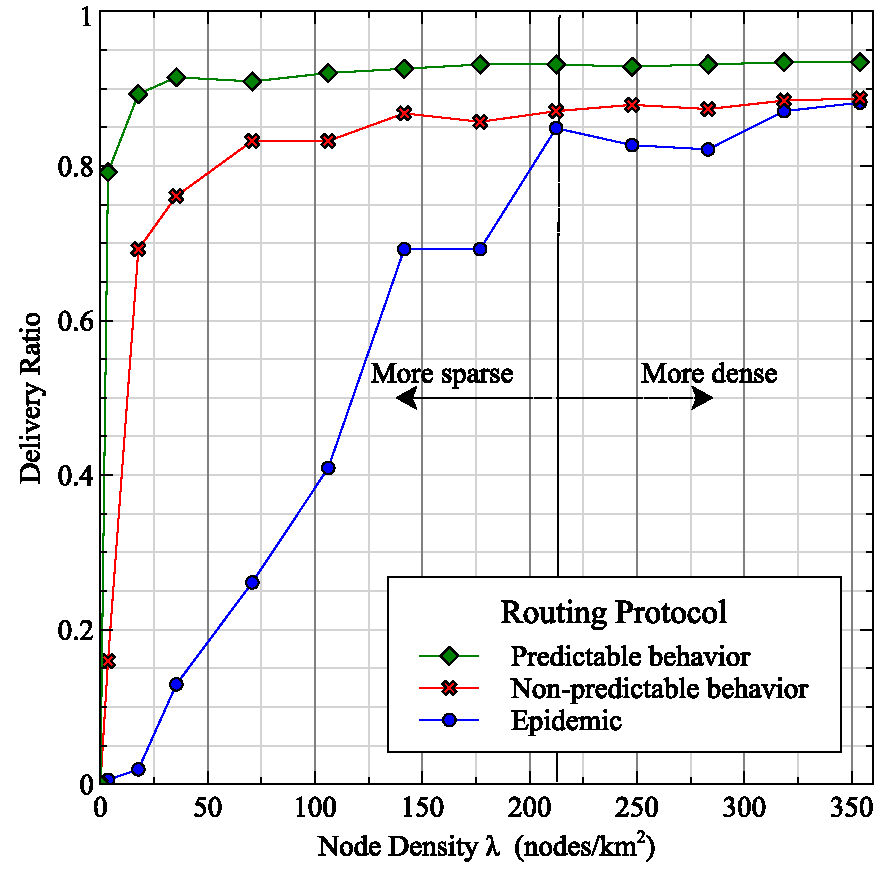
\includegraphics[width=2.5in]{Graphs/DeliveryRatio.pdf}
	\caption{Delivery Ratio per Node Density}
	\label{Delivery Ratio per Node Density}
\end{figure}

\begin{figure}[!t]
	\centering
	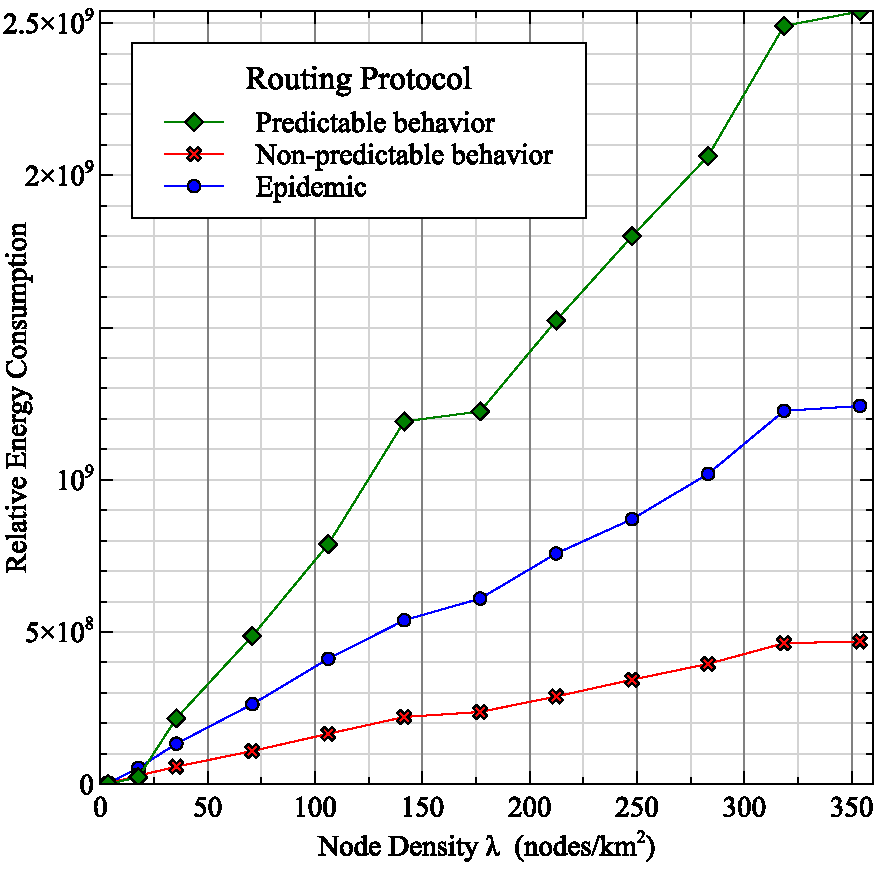
\includegraphics[width=2.5in]{Graphs/EnergyConsumption.pdf}
	\caption{Energy Consumption per Node Density}
	\label{Energy Consumption per Node Density}
\end{figure}

\begin{figure}[!t]
	\centering
	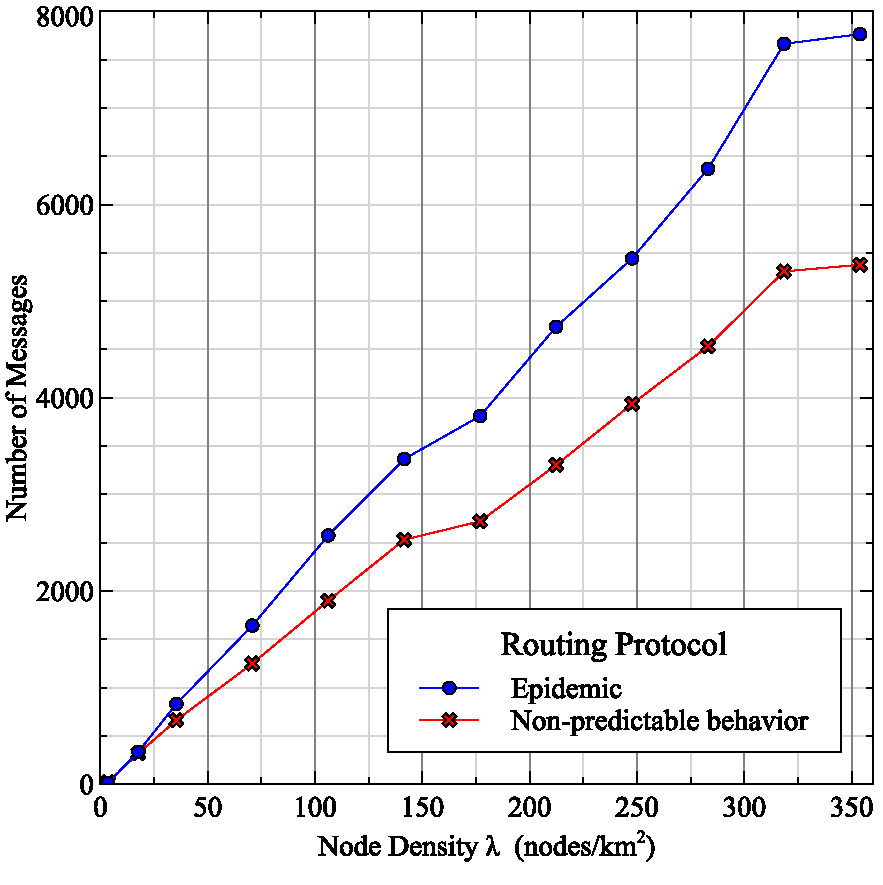
\includegraphics[width=2.5in]{Graphs/messages.pdf}
	\caption{Number of Generated Protocol Packets per Created Messages on Node Density}
	\label{Number of Generated Protocol Packets}
\end{figure}

\begin{figure}[!t]
\centering
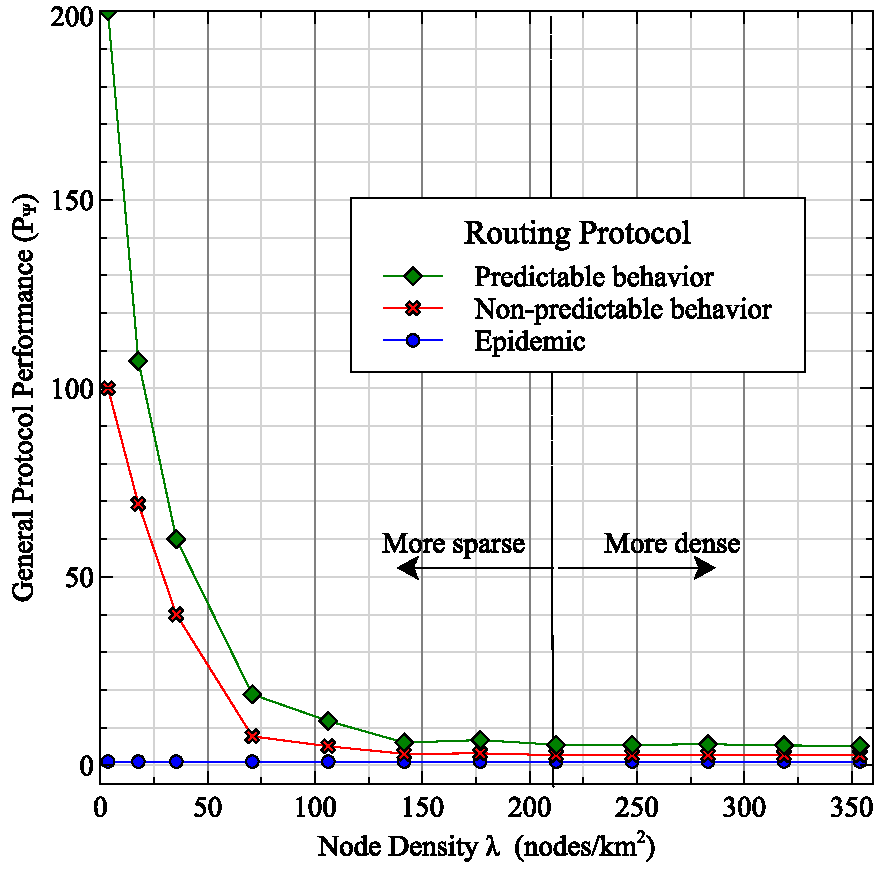
\includegraphics[width=2.5in]{Graphs/ProtocolPerformance.pdf}
\caption{General Protocol Performance per Node Density}
\label{General Protocol Performance per Node Density}
\end{figure}

Firstly, the comparison of delivery ratio is shown in Fig. \ref{Delivery Ratio per Node Density}, where $x-axis$ represents the node density (the number of nodes in the area of one $km^2$) and $y-axis$ shows the delivery ratio.
In our simulation, we assume the environment of one Rendezvous node and the ratio of time interval between full power and power saving, $\tau_s$ of 0.5.
%
Fig. \ref{Delivery Ratio per Node Density} shows that our proposed protocols gain slightly better delivery ratio in the dense environment.
On the other hand, the proposed protocols gain significantly higher delivery ratio in the sparse environment by maintaining the ratio up to 80\%, even when node density is as low as 50 $nodes/km^2$ in non-predictable behavior or as low as 5 $nodes/km^2$ nodes in predictable behavior.
Over all in average, our proposed protocols gain approximately 40\% higher delivery ratio than existing traditional Epidemic routing in sparse networks.

The reason behind the behaviors from this result is that the proposed Rendezvous concept can facilitate message exchanging process between nodes passing through the same area but on the different time-line as designed.
%%
Those nodes coincidence on both time and space domain are likely to happen more in dense network but will become rarely to happen when the network is more sparse.
%% 
In addition, with the knowledge of node gathering area (predictable behavior), the delivery ratio of the proposed protocol can be further increased especially in the extremely low node density. 

Secondly, the energy consumption ($E_c$), which is another vital factor in opportunistic network where most mobile nodes are usually equipped with limited power resources, is shown in Fig. \ref{Energy Consumption per Node Density}.
%%
The $x-axis$ represents node density and $y-axis$ is the $E_c$ in unit of energy consumption per 1,000 messages.
%%
This graph shows that the value of $E_c$ linearly increases when network become more dense.
%%
The trend on the graph is similar to the number of generated protocol packets per created messages on node density graph in Fig. \ref{Number of Generated Protocol Packets}.
%%
The predictable behavior save 80\% less energy consumption than Epidemic protocol while non-predictable behavior can save around 60\% of Epidemic counterpart.
%%
On the other hand, the number of generated protocol packets per created messages of predictable behavior is 60\% and for non-predictable behavior is 30\% lower than Epidemic protocol.
%%The reason for this behavior
The reason of $E_c$ rising in the dense environment results from the increasing of node meeting activities from growing number of nodes which generating more number of messages.
%
The trend similarity from Fig. \ref{Energy Consumption per Node Density} and \ref{Number of Generated Protocol Packets} is derived from the increasing number of messages in Eq. \ref{eq:enegy_consumed} which resulting in the rising in energy consumption. 
%%
Our proposed protocols require less number of generated messages while presenting significant lower $E_c$ which is the result from the fact that the Rendezvous protocols utilize less average wireless radius.

Combining both gains in delivery ratio and energy consumption saving, the proposed general protocol performance can be seen in Fig. \ref{General Protocol Performance per Node Density}. 
%
The Epidemic is used as the based-line protocol in $P_{\psi}$ calculation so its value in Fig. \ref{General Protocol Performance per Node Density} is 1.
%
The proposed protocol performance can achieve up to 20 times of the existing Epidemic when network is very sparse and on average about 5-10 times in general network environment.
al Epidemic protocol.

%%%%%%%%%%%%%%%%%%%%%%%%%%%%%%%%%%%%%%%%%%%%%%%%%%%%%%%%%%%%%%%%%%%%%%%%%%
\begin{figure}[!t]
\centering
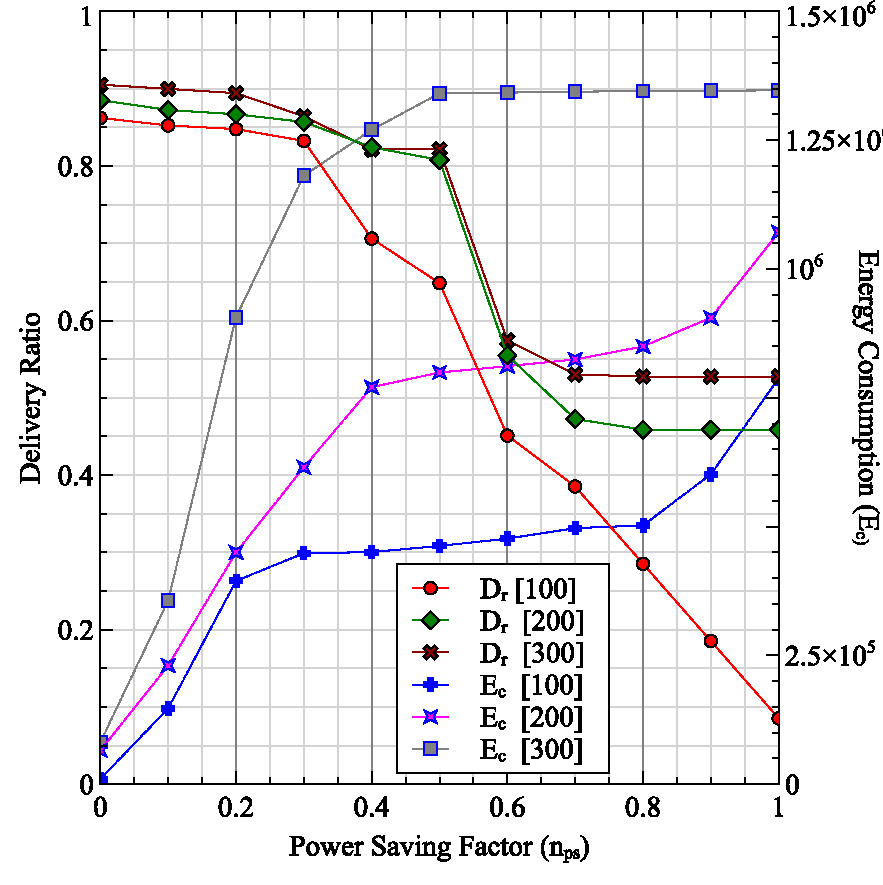
\includegraphics[width=2.5in]{Graphs/NpsDeliveryPerformanceAndDeliveryRatio.pdf}
\caption{Delivery Ratio and Energy Consumption on Power Saving Factor}
\label{The Optimum between Delivery Ratio and protocol Performance}
\end{figure}

\subsubsection{Impact from power saving factor}

In this subsection, we study protocol parameters relevant to the power saving factor and the trade-off between power consumption and delivery ratio.
%
We define the power saving factor, $n_{ps}$ as the composite parameters of the proposed protocol as in Eq. \ref{nps}.
%
\begin{equation}
{ n }_{ ps }={ \tau  }_{ s }\cdot \frac { { r }_{ c }^{ max }-{ r }_{ c }^{ min } }{ { r }_{ c }^{ max } } 
\label{nps}
\end{equation}
The $n_{ps}$ is mainly calculated from the time being in power saving mode, $\tau_s$ and the portion of energy consumption used when being in such power saving mode.
%
The value of $n_{ps}$ is in [0,1] range where its minimum value (no saving) represents either OppNet nodes never operate in power saving mode of the proposed protocol or the maximum energy consumption ($r_c^{min} = r_c^{max}$) is used in such mode.
%
The opposite behavior in power saving mode is for the maximum $n_ps$.
%
Fig. \ref{The Optimum between Delivery Ratio and protocol Performance} shows both delivery ratio ($D_r$ on solid line) and energy consumption ($E_c$ on dash line) when varying power saving factor ($n_{ps}$) for the node density ($\alpha$) = 100 and 300 $nodes/km^2$.
%
The graph shows that when $n_{ps}$ increases the value of $E_c$ and $D_r$ decreased as expected.
%
The delivery ratio for more sparse network significantly drops when the $n_{ps}$ increases because the saving factor can degrade the delivery performance if the nodes spend more time in saving mode.
%
In fact, the optimum of $n_{ps}$ depends on the real applications.
%
In the application with the level of acceptable minimum $D_r$ as a threshold, we can select the $n_{ps}$ that gives the minimum $E_c$.
%
On the other hand, we can select the $n_{ps}$ that gives the maximum $D_r$ if the threshold of acceptable maximum $E_c$ is defined.
%
Finally, if both the minimum $D_r$ and maximum $E_c$ are defined, we can get the $n_{ps}$ value that suit the application.

%%%%%%%%%%%%%%%%%%%%%%%%%%%%%%%%%%%%%%%%%%%%%%%%%%%%%%%%%%%%%%%%%%%%%%%%%%

\subsubsection{Other network environment parameters}

\begin{figure}[!t]
	\centering
	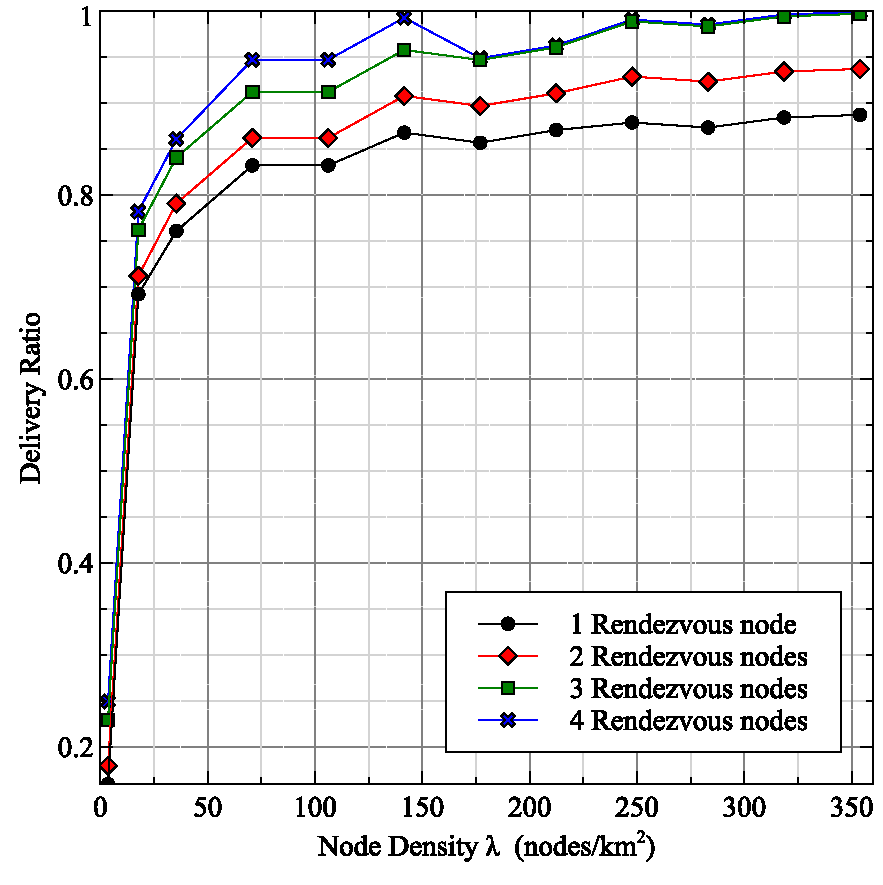
\includegraphics[width=2.5in]{Graphs/MultipleRVs.pdf}
	\caption{Multiple Rendezvous Nodes}
	\label{Multiple Rendezvous Nodes}
\end{figure}

\begin{figure}[!t]
\centering
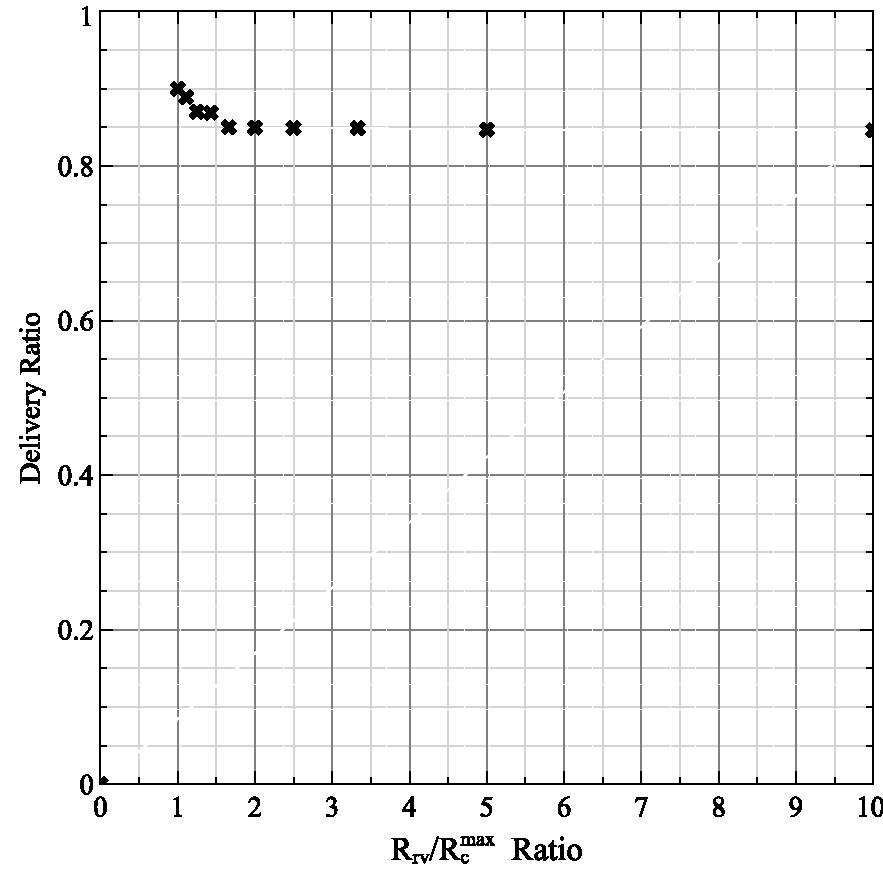
\includegraphics[width=2.5in]{Graphs/RcmaxRrv.pdf}
\caption{$R_{rv}$/$R_c^{max}$ ratio}
\label{RrvRcmaxRatio}
\end{figure}

\begin{figure}[!t]
\centering
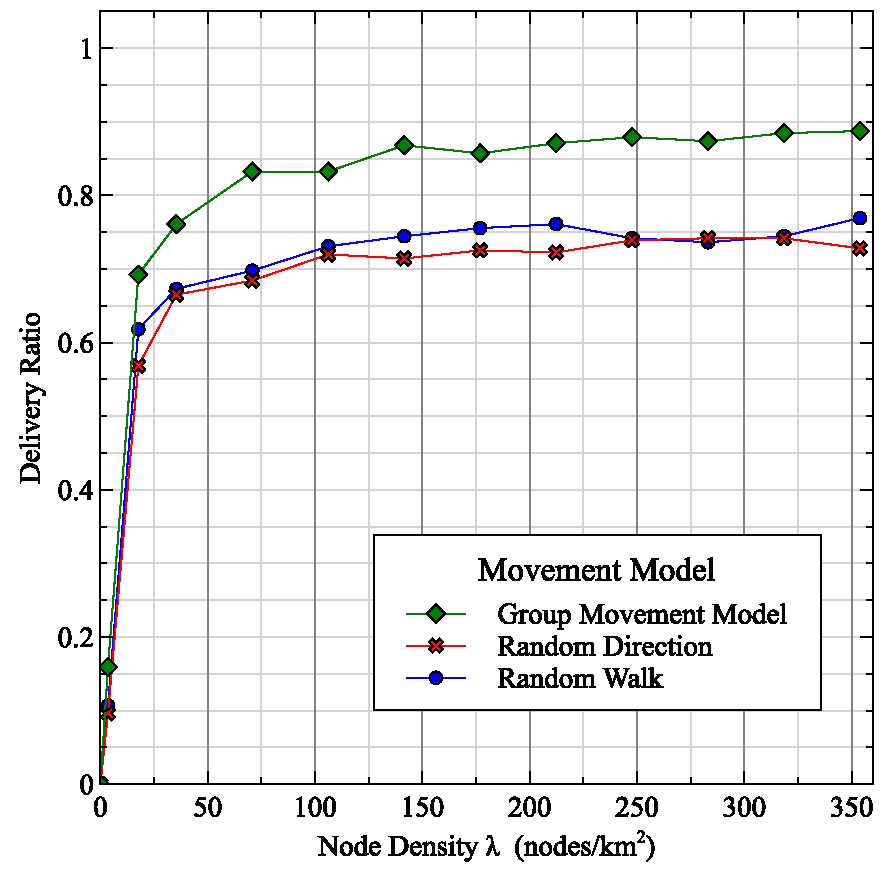
\includegraphics[width=2.5in]{Graphs/movement.pdf}
\caption{Movement Model Comparison}
\label{Movement Model Comparison}
\end{figure}

In this subsection, we investigate other protocol and environmental parameter which may have effect to the proposed protocol performance.
%
Fig. \ref{Multiple Rendezvous Nodes} presents the variation on the number of Rendezvous nodes to analyze the impact on delivery ratio per node density.
%
This graph shows that more Rendezvous nodes can achieve more $D_r$ as expected.
%
In Fig. \ref{RrvRcmaxRatio}, the effect of $R_{rv}/R_c^{max}$ ratio on delivery ratio is studied.
% 
By increasing $R_{rv}$ (maximum radio transmission of Rendezvous node), the $D_r$ will not increase but slightly decrease.
%
This is the result from the asymmetric in transmission range of OppNet nodes which can degrade the delivery ratio performance in Rendezvous area, since the nodes with longer transmission range can send the messages to other nodes with shorter range, but can not receive the messages back.
%%
Finally, Fig. \ref{Movement Model Comparison} shows that our proposed Rendezvous protocol performance will drop if node movement become more random since the proposed protocol utilizes the group gathering behavior to increase message exchanging activities.


\section{Conclusion}
Opportunistic Routing techniques can be applied in  plentiful variety of scenarios such as military network or wildlife monitoring. 
%
In this paper, we investigate the use of Rendezvous points in opportunistic network routing to increase the delivery ratio in extreme sparse network environment.
%
This novel protocol proposes the two new types of node, Rendezvous node and OppNet node, which can help maintaining the messages in one place as long as possible in order to bridge the gap of time and space domain.
%
In this Rendezvous place, the passing nodes can announce, deposit and pickup their own messages without meeting with other nodes that carried desired messages.
%
The size and shape of  Rendezvous place can be adapted to the environment of OppNet nodes in the area.
%
We define our routing model in two functions: predictable  and non-predictable behavior OppNet node functions.
%
The result suggest that our protocols perform significant higher in general protocol performance which is the trade off of delivery ratio per energy consumption.
%
We can simply imply that if the location of rendezvous place can be predicted, we can achieve highest overall performance.
%%
% Our experiment also suggest that the OppNet node can gain higher protocol performance when the time interval of power saving mode is longer and the minimum radio range is higher.
%%
In the future work, this concept of smart node can be further extend to increase the intelligence of the node since the technologies can be rapidly advanced.


\section*{Acknowledgment}
This work was supported by Sirindhorn International Institute of Technology, Thammasat University, Thailand and Basic Research Program from Data Communication Laboratory, Research and Development Department at Defense Technology Institute Thailand.

\bibliographystyle{IEEEtran}
\bibliography{RendezvousBib}
\end{document}


